\documentclass[12pt,spanish]{article}
\usepackage{beamerarticle}
\usepackage{babel}
\usepackage[utf8]{inputenc}
\usepackage{fullpage}
\usepackage{xcolor}
\usepackage{listings}
\usepackage{textcomp}
\usepackage{mathpazo}
\usepackage{courier}
\usepackage{fancyvrb}
\usepackage{amsmath}
\usepackage{url}
\usepackage{hyperref}
\usepackage{pgfpages}
\usepackage{wrapfig}
\usepackage{enumitem}

\hyphenation{sa-li-da}
\hyphenation{va-li-dar}

\lstset{xleftmargin=3em}

\newcommand{\onelinerule}{\rule[2.3ex]{0pt}{0pt}}
\newcommand{\twolinerule}{\rule[6.2ex]{0pt}{0pt}}
\newcommand{\respuesta}{\framebox[\textwidth]{\twolinerule}}
\newcommand{\nombre}{%
  \begin{tikzpicture}[xscale=.4,yscale=.7]
    \draw (0, 0) rectangle (22, 1);
  \end{tikzpicture}%
}
%\newcommand{\rol}   {\framebox[0.3\textwidth]{\onelinerule}}
\newcommand{\rol}{%
  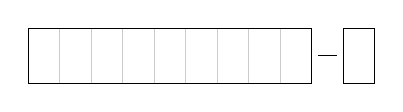
\begin{tikzpicture}[xscale=.4,yscale=.7]
    \draw[gray!40] ( 0, 0) grid      ( 9, 1);
    \draw          ( 0, 0) rectangle ( 9, 1);
    \draw          (10, 0) rectangle (11, 1);
    \draw (9 + .2, .5) -- (10 - .2, .5);
  \end{tikzpicture}%
}
\newcommand{\li}{\lstinline}
\newcommand{\pond}[1]{[{\small\textbf{#1\%}}]}

\lstdefinelanguage{py}{%
  classoffset=0,%
    morekeywords={%
      False,class,finally,is,return,None,continue,for,lambda,try,%
      True,def,from,nonlocal,while,and,del,global,not,with,print,%
      as,elif,if,or,yield,assert,else,import,pass,break,except,in,raise},%
    keywordstyle=\color{black!80}\bfseries,%
  classoffset=1,
    morekeywords={int,float,str,abs,len,raw_input,exit,range,min,max,%
      set,dict,tuple,list,bool,complex,round,sum,all,any,zip,map,filter,%
      sorted,reversed,dir,file,frozenset,open,%
      array,zeros,ones,arange,linspace,eye,diag,dot},
    keywordstyle=\color{black!50}\bfseries,%
  classoffset=0,%
  sensitive=true,%
  morecomment=[l]\#,%
  morestring=[b]',%
  morestring=[b]",%
  stringstyle=\em,%
}

\lstdefinelanguage{testcase}{%
  moredelim=[is][\bfseries]{`}{`},%
  backgroundcolor=\color{gray!20},%
}

\lstdefinelanguage{file}{%
  frame=single,%
  backgroundcolor=\color{white},%
}

\lstset{language=py}
\lstset{basicstyle=\ttfamily}
\lstset{columns=fixed}
\lstset{upquote=true}
\lstset{showstringspaces=false}
\lstset{rangeprefix=\#\ }
\lstset{includerangemarker=false}

\newlist{certamen}{enumerate}{1}
\setlist[certamen]{%
  label=\arabic*.,
  font=\LARGE\bfseries,%
  labelindent=-.5in,%
  leftmargin=0pt,%
  labelsep=1em%
}


\newcommand{\diapo}[1]{
  %\begin{wrapfigure}[11]{l}{.35\textwidth}
    \vspace{2ex}
    \fbox{\includeslide[width=.3\textwidth]{#1}}
  %\end{wrapfigure}
}


\title{Diapositivas y notas de clases}
\author{Programación \\ \url{http://progra.usm.cl}}
\date{}

\begin{document}
  \maketitle

  El material de clases de la asignatura de programación
  está compuesto por diapositivas y notas de clases.

  \section*{Diapositivas}

  Las presentaciones están diseñadas para apoyar una clase
  que consiste en presentación de contenidos,
  ejemplos y ejercicios para ser resueltos
  en la pizarra y en el computador.

  Las diapositivas no tienen texto en prosa para ser leído,
  sino que incluyen ejemplos, diagramas y enunciados de ejercicios,
  que el profesor puede usar como complemento para su exposición.

  No toda la información relevante a cada contenido
  aparece en las diapositivas,
  sino sólo la necesaria para presentar cada concepto.
  Para profundizar la materia y estudiar los detalles,
  es importante incentivar al estudiante
  para que lea el apunte del ramo y la bibliografía complementaria,
  busque en internet y ejercite por su cuenta.

  Cada profesor puede presentar los contenidos
  siguiendo su estilo personal,
  y apoyándose en la pizarra y el computador
  para desarrollar sus propios ejemplos.

  \section*{Notas de clases}
  Cada presentación va acompañada de un documento de notas de clases.

  Las notas no son una imposición para los profesores,
  sino más bien una explicación
  de cómo están pensadas las diapositivas para ser expuestas.
  Además, sirven como recordatorio para puntos importantes
  que es importante mencionar en clases
  y que podrían ser olvidados.

  \section*{Convenciones}

  Todos los programas y ejemplos que aparecen
  en apuntes, diapositivas y evaluaciones
  siguen todos algunas convenciones de estilo,

  Los ejercicios de hacer programas
  irán acompañados de casos de pruebas,
  que son un ejemplo de una ejecución del programa.
  Los casos de prueba tienen fondo gris
  y denotan la entrada del usuario con negrita:%
  \begin{lstlisting}[language=testcase,linewidth=.6\textwidth]
Ingrese anno de nacimiento: `1980`
Ingrese anno actual: `2011`
Usted tiene 31 annos.
  \end{lstlisting}

  Al desarrollar programas durante la clase,
  es conveniente apegarse al formato de salida del caso de prueba,
  pues es una manera muy clara de entender el enunciado
  y de validar la solución.
  Además, es el mismo formato que los estudiantes verán
  en certámenes, controles y laboratorios.

  El código fuente de programas aparece siempre
  con la sintaxis resaltada para mayor claridad:
  \begin{lstlisting}[language=py,linewidth=.5\textwidth]
nacimiento = int(raw_input('Ingrese anno de nacimiento: '))
actual     = int(raw_input('Ingrese anno actual: '))
edad = actual - nacimiento
print 'Usted tiene', edad, 'annos'
  \end{lstlisting}

  Los ejemplos que usan la consola interactiva
  pueden ser identificados por
  la aparición del símbolo \verb!>>>!:
  \begin{lstlisting}[language=py,linewidth=.5\textwidth]
>>> nacimiento = 1971
>>> actual = 2010
>>> actual - nacimiento
39
>>> edad = actual - nacimiento
>>> print edad
39
  \end{lstlisting}

  Los ejemplos interactivos pueden ser probados
  en vivo durante la clase,
  y complementados con variaciones y ejemplos adicionales.
  Esto resulta útil para hacer preguntas a los estudiantes
  y validar sus respuestas inmediatamente en el computador.

\end{document}


